% %& -job-name=weekly_report_200330_lutjens

\documentclass[letterpaper, 10 pt, conference, twocolumn]{ieeeconf}  % Comment this line out if you need a4paper
\IEEEoverridecommandlockouts                              % This command is only needed if 
\overrideIEEEmargins                                      % Needed to meet printer requirements.
%\pdfminorversion=4

% See the \addtolength command later in the file to balance the column lengths
% on the last page of the document
\usepackage{microtype}

% For videos
\usepackage{graphicx}
\usepackage{media9}


%\usepackage[sort,compress]{cite}%

\usepackage[pdftex,pdftitle={Template}]{hyperref}

\hypersetup{colorlinks,linkcolor={green!50!black},citecolor={green!50!black},urlcolor={black}, pdfauthor={Bj{\"o}rn L{\"u}tjens}}
\makeatletter \let\NAT@parse\undefined \makeatother
% \usepackage[square,comma,sort&compress]{natbib}
%\usepackage[sort,compress]{cite}

%\usepackage{subfigure,balance}
%\usepackage[colorlinks=true]{hyperref}
%\usepackage{algorithm} \usepackage[noend]{algorithmic}
\usepackage[linesnumbered,ruled,vlined]{algorithm2e}
\usepackage{multirow}

\usepackage{tabulary}
\newcolumntype{K}[1]{>{\centering\arraybackslash}p{#1}}

\newtheorem{definition}{Definition}
\newtheorem{assumption}{Assumption} \newtheorem{theorem}{Theorem}
\newtheorem{lemma}{Lemma}
\newtheorem{corollary}[theorem]{Corollary}

\iffalse
\newif\ifPDF \ifx\pdfoutput\undefined\PDFfalse \else\ifnum\pdfoutput > 0\PDFtrue \else\PDFfalse \fi \fi

\ifPDF
\usepackage[pdftex, pdfstartview={FitV}, pdfpagelayout={TwoColumnLeft},bookmarksopen=true,plainpages = false, colorlinks=true, linkcolor=black, citecolor = black, urlcolor = black,filecolor=black, pagebackref=false,hypertexnames=false, plainpages=false, pdfpagelabels ]{hyperref}
\fi


\usepackage{float}
%\usepackage[numbers,sort&compress]{natbib}  % Might want to use this one.....
%\usepackage{hypernat}

%% IEEE bib style
\makeatletter
\def\bstctlcite#1{\@bsphack
  \@for\@citeb:=#1\do{%
    \edef\@citeb{\expandafter\@firstofone\@citeb}%
    \if@filesw\immediate\write\@auxout{\string\citation{\@citeb}}\fi}%
  \@esphack}
\makeatother

\title{\LARGE \bf Uncertainty quantification in physics-informed neural networks \\ 16.940 Final Project}

\author{Bj{\"o}rn L{\"u}tjens (lutjens@mit.edu, 912238433)% <-this % stops a space
\thanks{\hspace*{-.17in} 16.940 Numerical Methods for Stochastic Modeling, Human Systems Laboratory, Massachusetts Institute of Technology, 77 Mass.\ Ave., Cambridge, MA, USA {\tt\footnotesize \{lutjens\}@mit.edu}}%
}


% \usepackage[usenames]{color}
%\DeclareMathOperator*{\argmin}{arg\,\!min}
%\DeclareMathOperator*{\argmax}{arg\,\!max}

% Redefine subsubsection command
\makeatletter
\renewcommand\paragraph{\@startsection{subsubsection}{4}{\z@}%
{0.25ex \@plus.5ex \@minus.2ex}%
{-.15em}%
{\normalfont\normalsize\itshape}}
\makeatother


%\usepackage{graphics} % for pdf, bitmapped graphics files
\usepackage{graphicx} % more modern
%\usepackage{epsfig} % for postscript graphics files
\usepackage{amsfonts}
\usepackage{amsmath,soul}
\usepackage{amssymb}
\usepackage[capitalize]{cleveref} %cref
%\crefformat{equation}{(#2#1#3)}%
%\Crefformat{equation}{Equations~(#2#1#3)}
%\Crefname{equation}{Equation}{}

\usepackage{dsfont} % mathds
\usepackage[font=small,skip=0pt]{subcaption} %subfigure
\usepackage{balance}
\usepackage[font=small]{caption}
\usepackage{bm} % bold italic vectors
\usepackage{wrapfig}
\usepackage{float} % To place figure on top right as float

% Define special colors
\usepackage{color}
\usepackage[svgnames]{xcolor} \definecolor{DarkGreen}{rgb}{0,0.5,0}
\definecolor{DarkRed}{rgb}{0.75,0,0}

% Define author comments
\usepackage[authormarkuptext=name,addedmarkup=bf,authormarkupposition=left]{changes}
%\usepackage[final]{changes} %Use this to hide all comments.
\definechangesauthor[name={J.~H.}, color={blue}]{jh}
\definechangesauthor[name={M.~E.}, color={red}]{me}
\definechangesauthor[name={B.~L.}, color={green}]{bl}
\setlength {\marginparwidth }{2cm}
\newcommand{\XX}[1]{\added[id=jh,remark={}]{#1}}
\newcommand{\meXX}[1]{\added[id=me,remark={}]{#1}}
\newcommand{\blXX}[1]{\added[id=bl,remark={}]{#1}}
\newcommand{\jsec}[1]{\marginpar{\fcolorbox{yellow}{yellow}{\parbox{0.7in}{\raggedright
        \color{blue} \tiny #1 }}}}
\newcommand{\hsec}[1]{\marginpar{\fcolorbox{yellow}{yellow}{\parbox{0.7in}{\raggedright
        \color{green} \tiny #1 }}}}
\newcommand{\jhmargin}[2]{{\color{orange}#1}\marginpar{\color{red}\tiny\raggedright
    \bf [JH] #2}}

% tikz
\usepackage{tikz,mathtools}
\crefformat{equation}{(#2#1#3)}
\Crefformat{equation}{Equation~(#2#1#3)}
\Crefname{equation}{Equation}{Equations}
\newcommand{\inputTikZ}[2]{\scalebox{#1}{\input{#2}}}
\usetikzlibrary{shapes,positioning,automata,arrows,fit,backgrounds,calc}
\tikzstyle{block} = [draw, fill=blue!20, rectangle,minimum height=1em,
minimum width=2em] \tikzstyle{sum} = [draw, fill=blue!20, circle, node
distance=1cm] \tikzstyle{input} = [coordinate] \tikzstyle{output} =
[coordinate] \tikzstyle{pinstyle} = [pin edge={to-,thin,black}]
\usetikzlibrary{trees} \usetikzlibrary{decorations.pathmorphing}
\usetikzlibrary{decorations.markings}
\definecolor{darkgreen}{rgb}{0,0.5,0}
\definecolor{darkred}{rgb}{220,20,60}

% Define argmin argmax
\DeclareMathOperator*{\argmin}{\arg\!\min}
\DeclareMathOperator*{\argmax}{\arg\!\max}

% Single line comment
\newcommand{\cmmnt}[1]{\ignorespaces}

% Define commands for itemized lists
\newcommand{\bit}{\begin{itemize}}
\newcommand{\ei}{\end{itemize}}


\begin{document}

% Import IEEE citation style
%\bstctlcite{IEEEexample:BSTcontrol}

\maketitle
\thispagestyle{empty}
\pagestyle{empty}
%%%%%%%%%%%%%%%%%%%%%%%%%%%%%%%%%%%%%%%%%%%%%%%%%%%%%%%%%%%%%%%%%%%%%%%%%%%%%%%%
\iffalse
\begin{abstract}
\end{abstract}
\fi
\section{Introduction}\label{sec:intro}

Decision-makers require uncertainty-expressive climate projections to accurately manage climate risks; for example, to take high-stake decisions for building climate-resilient infrastructure. The quantification of uncertainty in local climate projections, however, requires ensemble forecasts of global climate models which are computationally very expensive. To reduce computational cost, global climate models use parameters to capture small-scale dynamics such as cloud formation that happen below the computationally feasible grid resolution~\cite{Yuval_2020}. These parameters, called subgrid parametrizations, are often based on physical intuition or low-dimensional function approximators, which can introduce substantial uncertainties in the global climate projections~\cite{Yuval_2020}. 

Recent works, explores high-dimensional function approximators such as random forests~\cite{Yuval_2020} or neural networks~\cite{Rackauckas_2020} to approximate the subgrid parametrizations from computationally expensive models that resolve the small-scale dynamics (e.g., cloud-resolving models). When approximating subgrid-parametrizations, however, it is important to accurately model the uncertainty in the parameter to support downstream risk management decisions. 

Zhang et al., 2019~\cite{Zhang_2019} estimates parameters, i.e., solves the inverse problem, by estimating the modes/coefficients of an arbitrary polynomial chaos expansion (PCE) as with neural networks. This paper strives towards the reimplementation of~\cite{Zhang_2019}\footnote{no source code was found online} and consists of four sections: 
\bit
  \item (II) Set up a stochastic diffusion equation and an approximation with PCE
  \item (III) Estimate the PCE coefficients from manually derived PCE coefficients
  \item (IV) Estimate the PCE coefficients from measurements of the diffusion parameter
  \item (V) Discussion of physics-informend neural networks, model uncertainty, and climate modeling
  \iffalse
  ~\cite{Zhang_2019} to generate summaries of the parameter in the 1D elliptic stochastic diffusion equation, as detailed in project 1,2, and~\cref{sec:1}.
  \item (1) Reimplement~\cite{Zhang_2019} to generate summaries of the parameter in the 1D elliptic stochastic diffusion equation, as detailed in project 1,2, and~\cref{sec:1}.
  \item (2) Discuss the quality of~\cite{Zhang_2019} in comparison to the Karhunen-Loeve expansion and polynomial chaos expansion from project 2.  
  \item (3) Discuss the quality the underlying approximation to Bayesian neural networks, called MC-Dropout~\cite{Gal_2016, Verdoja_2020}. 
  \item (4) Analyse assumptions of~\cite{Zhang_2019} and discuss the applicability to an equation from climate modeling, e.g., a 1D advection-diffusion equation\cite{Rackauckas_2020} or large eddy simulations~\cite{Souza_2020,Sarghini_2003}  
  \fi
\ei

\section{Target: 1D elliptic stochastic diffusion equation}\label{sec:1}
\subsection{Defining the stochastic diffusion equation}\label{sec:sde}
\begin{figure}[h]
    \centering
    \begin{minipage}[b]{.6\linewidth}
    \centering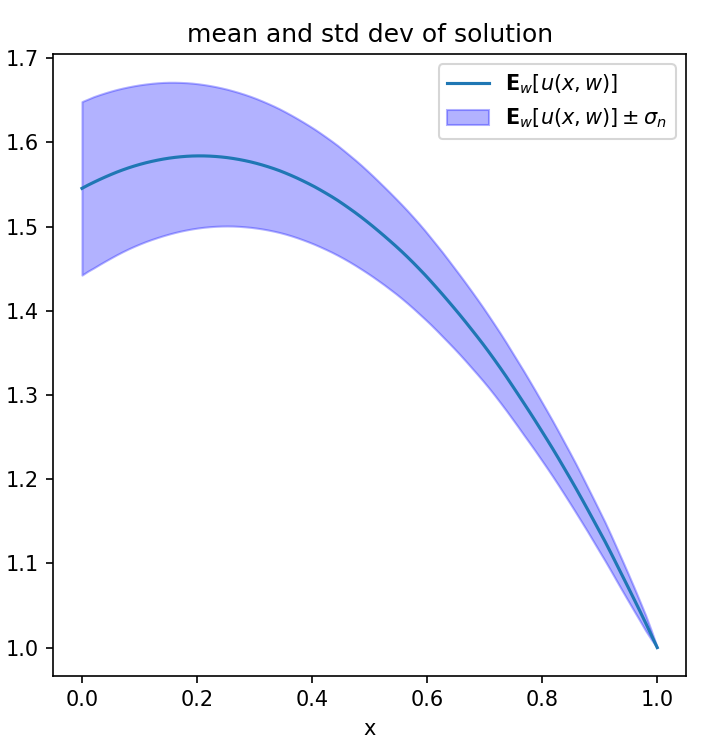
\includegraphics [trim=0 0 0 0, clip, width=0.9\textwidth, angle = 0]{figures/solution_1d_elliptic_sde}
    \end{minipage}% 
\caption{Solution to the 1D elliptic stochastic diffusion equation}\label{fig:solution_1d_sde}
\end{figure}

Similar to project 1, we are given the 1D elliptic stochastic diffusion equation
\begin{equation}
\begin{aligned}
  \frac{\delta}{\delta x}(k(x,\omega) \frac{\delta u(x,\omega)}{\delta x}) &= -s(x),\\
\end{aligned} 
\label{eq:sde}
\end{equation}
with location, $x \in D = [0,1]$, noise, $\omega \in \Omega$, solution, $u:D\times\Omega \rightarrow \mathds R$, diffusivity, $k: D\times\Omega \rightarrow \mathds R$, and source, $s(x)=5$. The solution of the stochastic diffusion equation is displayed in~\cref{fig:solution_1d_sde}. The stochastic diffusion equation has a deterministic Dirichlet boundary condition at $x=1$

\begin{equation}
\begin{aligned}
  u(x=1,\omega) = u_r = 1, \\
\end{aligned}  
\label{eq:dirichlet}
\end{equation}
and a random Neumann condition at $x=0$:
\begin{equation}
\begin{aligned}
  k(x, \omega)\frac{\delta u}{\delta x}\rvert_{x=0} = -F(\omega), \\
\end{aligned}  
\label{eq:neumann}
\end{equation}
with Flux, $F(\omega) \sim \mathcal N(\mu_F=-1.0, \sigma_F^2=0.2)$. 

\subsection{Defining the target: polynomial chaos expansion coefficients}\label{sec:sde}
The diffusivity is stochastic assumed to be the unknown subgrid parameterization and will be approximated by an approximate Bayesian neural network. The diffusivity is assumed to follow a Gaussian Process (GP), $Y(x,\omega)$, with $k(x,\omega)=\exp(Y(x, \omega))$. The GP is defined by mean, $\mu_Y=1.0$, correlation length, $L=0.3$, variance, $\sigma_Y^2=0.3$, exponent, $p_{GP}=1.0$, and a covariance kernel that is similar to the non-smooth ornstein-uhlenback kernel:
\begin{equation}
\begin{aligned}
  C(x_1, x_2) = \sigma_Y^2 \exp(-\frac{1}{p_{GP}} (\frac{\lvert x_1 - x_2 \rvert}{L})^p).\\
\end{aligned}  
\label{eq:kernel}
\end{equation}

The Gaussian Process is further disentangled into deterministic spatial domain and stochastic domain via a polynomial chaos expansion (PCE), similar to project 2. The PCE approximates the diffusivity as a linear combination of the PCE coefficients, $C_{\vec\alpha}(x)$, and the a set of polynomials, $\Psi_{\vec\alpha}(\xi_1,...\xi_n)$. The PCE is then calculated as follows:
\begin{equation}
\begin{aligned}
Y(x) &= \sum_{\alpha_1=0}^\infty\sum_{\alpha_2=0}^\infty...\sum_{\alpha_n=0}^\infty C_{(\alpha_1, ..., \alpha_n)}(x)\Psi_{(\alpha_1, ..\alpha_n)}(\xi_1, ..., \xi_n)\\
\approx \hat Y(x) &= \sum_{\vec\alpha\in\{\lvert\lvert\vec\alpha \rvert\rvert_1 \leq n\}} C_{\vec\alpha}(x) \Psi_{\vec\alpha}(\xi_1, ..., \xi_n), \\
\end{aligned}
\label{eq:pce}
\end{equation}
The set of polynomials is a set of multivariate orthogonal Gaussian-Hermite polynomials, 
\begin{equation}
\begin{aligned}
\Psi_{\vec \alpha}(\xi_1, ..., \xi_n) &= \Pi_{i=1}^n \psi_{\alpha_i}^{(i)}(\xi_i),\\
&= \Pi_{i=1}^n \text{He}_{\alpha_i}^{(i)}(\xi_i), \\
\text{with } \xi_i &\sim \mathcal{N}(0,1).
\end{aligned}
\label{eq:gauss_herm_poly}
\end{equation}
Each polynomial, $\text{He}_{\alpha_i}(\xi_i)$, has the polynomial degree, $\alpha_i$, given by the total-degree multi-index set, $A=\{\vec \alpha \in \mathds{N}_0^{n}: \lvert \lvert \vec \alpha \rvert\rvert_1 = \sum_{j=1}^n\alpha_j \leq n\}$. Throughout this write-up the maximum polynomial degree is $n=3$.
\begin{figure}[t]
    \centering
    \begin{minipage}[b]{0.8\linewidth}
    \centering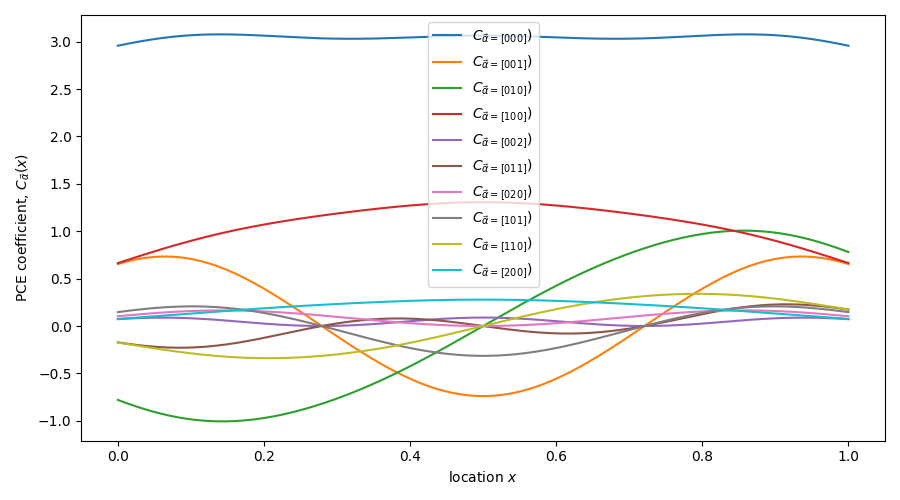
\includegraphics [trim=0 0 0 0, clip, width=0.9\textwidth, angle = 0]{figures/pce_poly_deg_3/pce_coefs}
    \subcaption{Target PCE coefficients with $n=3$ over $x$.}\label{fig:pce_coefs}
    \end{minipage}% 
    \\
    \begin{minipage}[b]{0.9\linewidth}
    \centering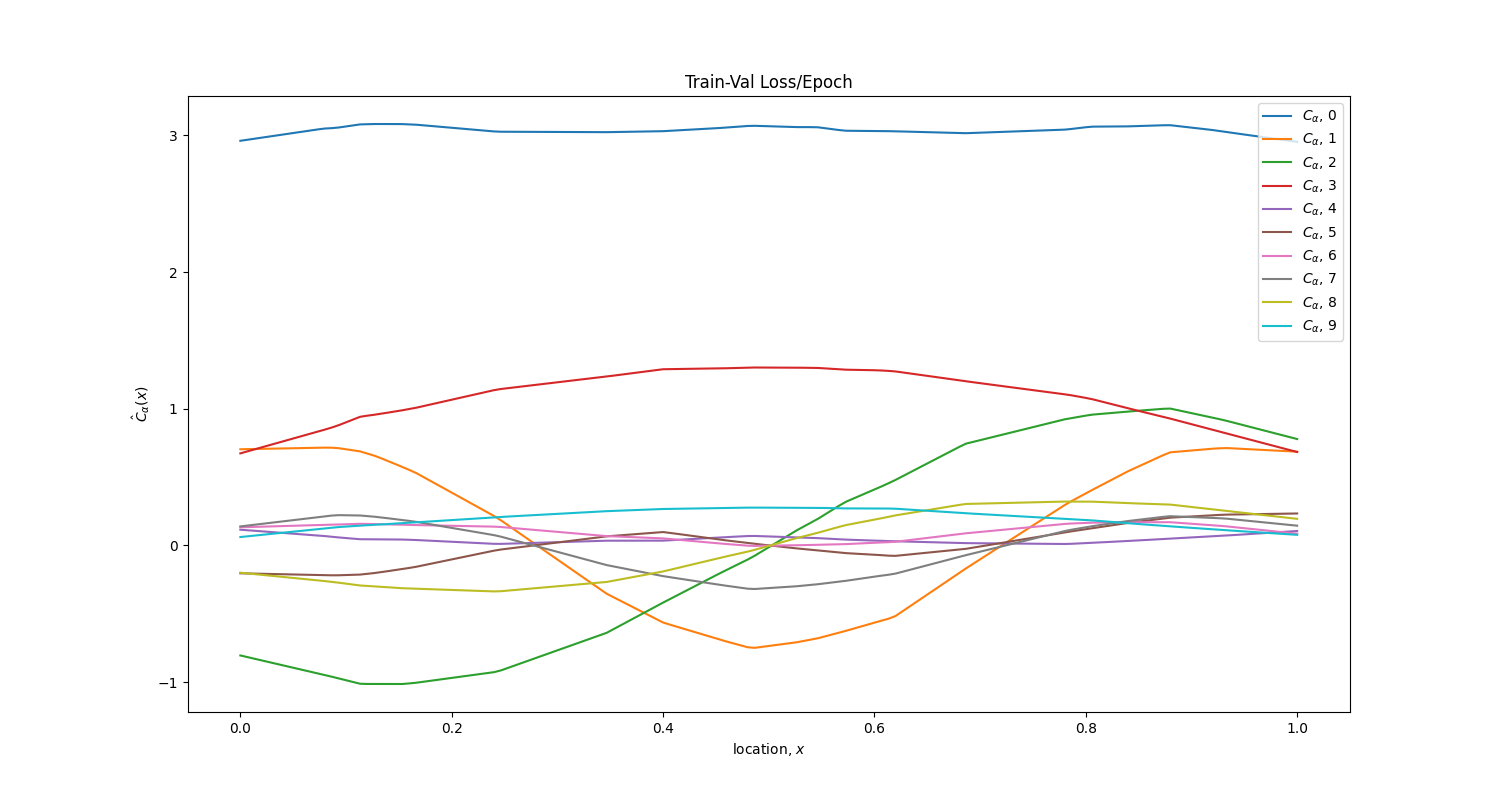
\includegraphics [trim=0 0 0 0, clip, width=0.9\textwidth, angle = 0]{figures/est_pce_coefs_nn/nn_pce_coefs}
    \subcaption{Learned PCE coefficients.}
    \label{fig:nn_pce_coefs}
    \end{minipage}% 
\caption{The learned PCE coefficients (bot) match the target coefficients (top) with MSE$\approx 0.0007$, but are less smooth.}
\label{fig:all_pce_coefs}
\end{figure}
Computing the PCE coefficients, $C_{\vec\alpha}(x)$, is typically computationally expensive. The ground-truth coefficients are shown in~\cref{fig:pce_coefs} and have been computed by approximating the Gaussian Process by a Karhunen-Lóeve-expansion and computing:
\begin{equation}
\begin{aligned}
  C_{\vec \alpha}(x_i) &= \frac{<\exp(Y(x_i)), \Psi_{\vec\alpha}(\xi_1, ..., \xi_n)>}{\lvert\lvert\Psi_{\vec\alpha}(\xi)\rvert\rvert_{L^2_{\mu_\xi}}^2}, \;\;\;\; \\
\end{aligned}
\label{eq:pce_coef}
\end{equation}
The nominator has been calculated as: 
\begin{align}
  &<\exp(Y(x_i)), \Psi_{\vec\alpha}(\xi_1, ..., \xi_n)>, \label{eq:nom_kl}\\
   &\approx <\exp(\mu_Y + \sum_{j=1}^{n}\sqrt{\lambda_j} \phi_j(x_i) \xi_j), \Psi_{\vec\alpha}(\xi_1, ..., \xi_n)>,\label{eq:nom_exp}\\
   &= \int_{-\infty}^{\infty}\exp(\mu_Y + \sum_{j=1}^n\sqrt{\lambda_j} \phi_j(x_i) \xi_j)\nonumber\\& \Pi_{j=1}^n \text{He}_{\alpha_j}(\xi_j)p(\xi_1,...,\xi_n) d\xi_1 ... d\xi_n,\label{eq:nom_iid}\\
   &= \exp(\mu_Y) \Pi_{j=1}^n \int_{-\infty}^{\infty} \exp(\sqrt{\lambda_j} \phi_j(x_i) \xi_j) \text{He}_{\alpha_j}(\xi_j)p(\xi_j)d\xi_j,\label{eq:nom_gauss_herm}\\
   &\approx \exp(\mu_Y) \Pi_{j=1}^n \sum_{k=0}^{n_\text{quad}} \exp(\sqrt{\lambda_j} \phi_j(x_i) \zeta_k) \text{He}_{\alpha_j}(\zeta_k)\omega_k
\end{align}
, where~\cref{eq:nom_kl} uses the KL-expansion,~\cref{eq:nom_exp} expands the norm,~\cref{eq:nom_iid} assumes that $\xi_j$ are independent,~\cref{eq:nom_gauss_herm} uses the Gauss-Hermite quadrature rule at $n_{quad}=n^2$ quadrature points, $\zeta_k$, with quadrature weights, $\omega_k$, for integration. 

The denominator has been calculated as, 
\begin{align}
  &\lvert\lvert\Psi_{\vec\alpha}(\xi)\rvert\rvert_{L^2_{\mu_{\vec\xi}}}^2, \nonumber\\
  &= <\Psi_{\vec\alpha}(\xi_1, ..., \xi_n), \Psi_{\vec\alpha}(\xi_1, ..., \xi_n)>, \label{eq:denom_norm}\\
   &=\int_{-\infty}^{\infty} \Pi_{i=1}^n\;\psi_{\alpha_i}(\xi_i)\Pi_{j=1}^n\;\; \psi_{\alpha_j}(\xi_j)\;p_{\xi_1,...\xi_n}(\xi_1,...,\xi_n)d\xi_1...d\xi_n\label{eq:denom_orth},\\
   &=\int_{-\infty}^{\infty} \; \Pi_{j=1}^n(\psi_{\alpha_j}(\xi_j)\psi_{\alpha_j}(\xi_j)\delta_{jj})\;p_{\xi_1,...\xi_n}(\xi_1,...,\xi_n)d\xi_1...d\xi_n\label{eq:denom_iid},\\
   &=\Pi_{j=1}^n\int_{-\infty}^{\infty} \;\psi_{\alpha_j}(\xi_j) \psi_{\alpha_j}(\xi_j)\;p_{\xi_j}(\xi_j)d\xi_j\label{eq:denom_gauss_herm}\\
   &=\sqrt{2\pi}\Pi_{j=1}^n\alpha_j!,
\label{eq:denom_pce}
\end{align}
where~\cref{eq:denom_norm} expands the norm,~\cref{eq:denom_orth} assumes that $\psi_j$ are orthonormal, assumes that $\xi_j$ are independent,~\cref{eq:denom_gauss_herm} assumes that $\psi_j$ is Hermite and $\xi_j$ Gaussian. 


\section{Learning PCE coefficients from analytically derived targets}\label{sec:learn_pce_coefs1}
The computation of PCE coefficients can be computationally expensive, arduous, and error-prone. Approximating the polynomial coefficients from data could alleviate this difficulty.  Hence, the following experiments to estimate the PCE coefficients from data.
\subsection{Approach}
First, a neural network, $NN_{C_{\vec\alpha}}(x)=\hat C_{\vec\alpha}(x):\mathds [x_\text{min},x_\text{max}] \rightarrow \mathds R^{\lvert A \rvert}$, is trained to approximate PCE coefficients while using the analytically derived PCE coefficients, $C_{\vec\alpha}(x)$, as target. The loss function for parameter, $C$, at episode, $e$, and batch, $b$, is defined as:
\begin{equation}
\begin{aligned}
  L_{C,e}(x_b) &= \frac{1}{B}\sum_{b=1}^B \lvert\lvert \sum_{\vec\alpha\in A}C_{\vec\alpha}(x_b) - \hat C_{\vec\alpha}(x_b)\rvert\rvert_2^2\\
\end{aligned}
\label{eq:loss_k}
\end{equation}


\subsection{Results}
\Cref{fig:nn_pce_coefs} shows the learned PCE coefficients and~\cref{fig:nn_k} shows corresponding diffusion, $k=exp(Y)$. The learned PCE coefficients match the target PCE coefficients very well, quantified by a low  $\text{MSE}_{C_{\vec\alpha}} = \frac{1}{E}\sum_e^E L_{C,e} \approx 0.0007$. The learned coefficients are less smooth, but based on further experiments increasing the network size smoothes the function (not shown). This good performance of the neural network is expected, because the PCE coefficients are a deterministic target and neural networks are a universal function approximator. 

The neural network, $NN_{C_{\vec\alpha}}(x)$ has a fully-connected, 6-layer, $1\times 16\times 32\times 64\times 64\times 32\times 16 \times \lvert A \rvert$-unit network, trained with ADAM with learning rate $0.001$, $\beta=[0.9,0.999]$, batch size $10$, number of epochs $30$, with loss function, $\text{MSE}_{C_{\vec\alpha}}$, implemented in the automatic differentiation library, pyTorch.
\begin{figure}[t]
    \centering
    \begin{minipage}[b]{0.7\linewidth}
    \centering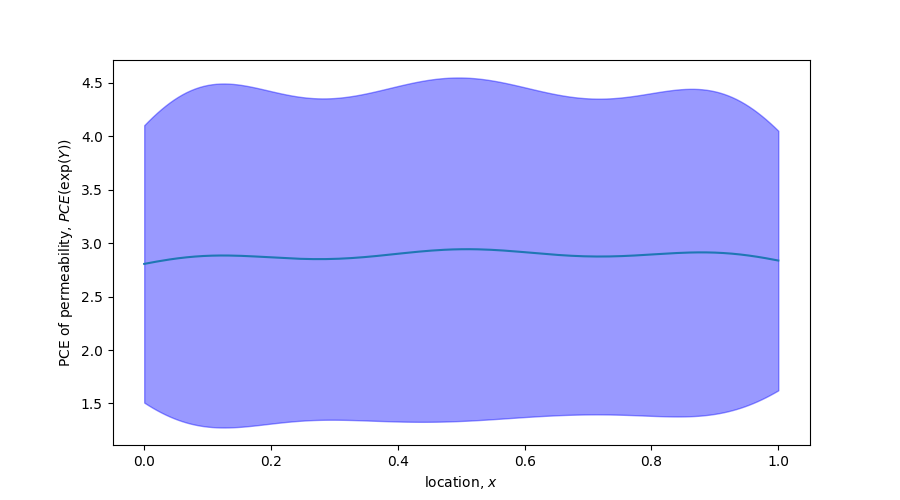
\includegraphics [trim=0 0 0 0, clip, width=0.9\textwidth, angle = 0]{figures/pce_poly_deg_3/pce_exp_of_y}
    \subcaption{Estimated diffusion from target PCE coefficients.}\label{fig:target_k}
    \end{minipage}% 
    \\
    \begin{minipage}[b]{0.7\linewidth}
    \centering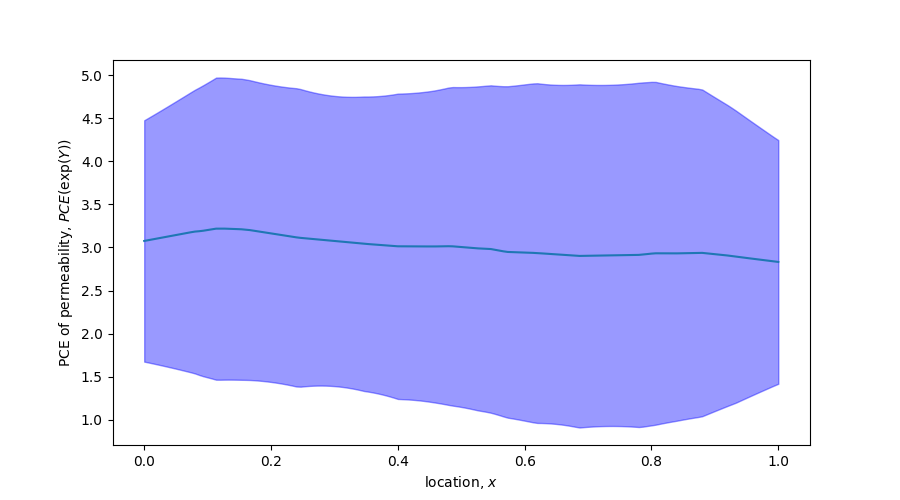
\includegraphics [trim=0 0 0 0, clip, width=0.9\textwidth, angle = 0]{figures/est_pce_coefs_nn/pce_exp_of_y}
    \subcaption{Estimated diffusion from learned PCE coefficients.}\label{fig:nn_k}
    \end{minipage}% 
\caption{Estimated diffusion, $k=\exp(Y)$, from target (top) and learned (bot) PCE coefficients.}
\label{fig:k}
\end{figure}

\section{Learning PCE coefficients from diffusion data}\label{sec:coef_data}
The previous training set-up still requires the estimation of the PCE coefficients via computationally expensive calculation. Thus, we are assuming now that measurements of the diffusion parameter, $k=\exp(Y)$, exist and infer PCE coefficients from this data. The loss function for parameter, $k$, per episode, $e$, then becomes:
\begin{equation}
\begin{aligned}
  L_{k,e} &= \frac{1}{B}\sum_{b=1}^B \lvert\lvert k_b - \hat k_{\vec\alpha}\rvert\rvert_2^2\\
  &= \frac{1}{B}\sum_{b=1}^B \lvert\lvert k_b - \exp(\sum_{\alpha \in A} \hat C_{\vec\alpha}(x_b)\Psi_{\vec\alpha}(\xi_1, ..., \xi_n))\rvert\rvert_2^2\\
\end{aligned}
\label{eq:loss_k}
\end{equation}
The deterministic neural network approximates the correct mean, but not the variance, as shown in~\cref{fig:est_k_nn} (bot). The poor fit is quantified by the low $\text{MSE}_k = \frac{1}{E}\sum_e^E L_{k,e}\approx 2.4$. The low variance can due to various reasons:

First, the stochasticity in predictions is averaged out during calculation of the loss function. One could overcome this effect by using the same realizations of the random variables $\xi_i$ for generation of the train and test dataset. However, one could not apply this set-up to real-world measurements. 

Second, the neural network approximates all PCE coefficients as zero except for the coefficient of the zero-th order polynomials, $C_{[0,0,0]}$, shown in~\cref{fig:est_k_nn} . Because the zero-th order polynomials are constant, $\text{He}_0(\xi)=1\forall \xi$, there cannot be variance in the generated diffusion, $k$. However, further experiments have shown that removing the zero-th order from the set of possible polynomials does not enable stochastic predictions. 

I would have expected this experiment to estimate the stochasticity, because the experiment in~\cite{Zhang_2020} is very similar. Greater inspection needs to done to identify how they overcame the issue of a deterministic forecast. 

Also, the training set-up removed spatial dependence due to the computational expense. The spatial dependence was removed by assuming that each sample-pair, $[x_b,k_b]$, in the batch of size, $B$, is independent. The spatial dependence could be reintroduced by extending the neural network domain to the full input domain $NN_{C_{\vec\alpha}}(x):\mathds R^{n_{\text{grid}}} \rightarrow \mathds R^{n_{\text{grid}}\times \lvert A\rvert}$. Expanding the domain requires a significantly larger neural network, which was computationally infeasible during this project. However, deep neural networks excel in areas of high-dimensional input spaces, e.g., high-resolution image-to-image-translation~\cite{Isola_2017} and I would expect the neural networks to be computationally feasible and accurate. For the task, so far, simpler regression models such as multivariate linear regression, SVM, or random forests would have probably sufficed, but a subgoal of the write-up was to show feasibility of scalable neural networks. 

The hyperparameters in this set-up where the same as in~\cref{sec:learn_pce_coefs1}, except for batch size, $B=1000$, and number of epochs, $E=100$. The training and test set, $k$, contained each $1000$ samples.
\begin{figure}[h!]
    \centering
    \begin{minipage}[b]{0.7\linewidth}
    \centering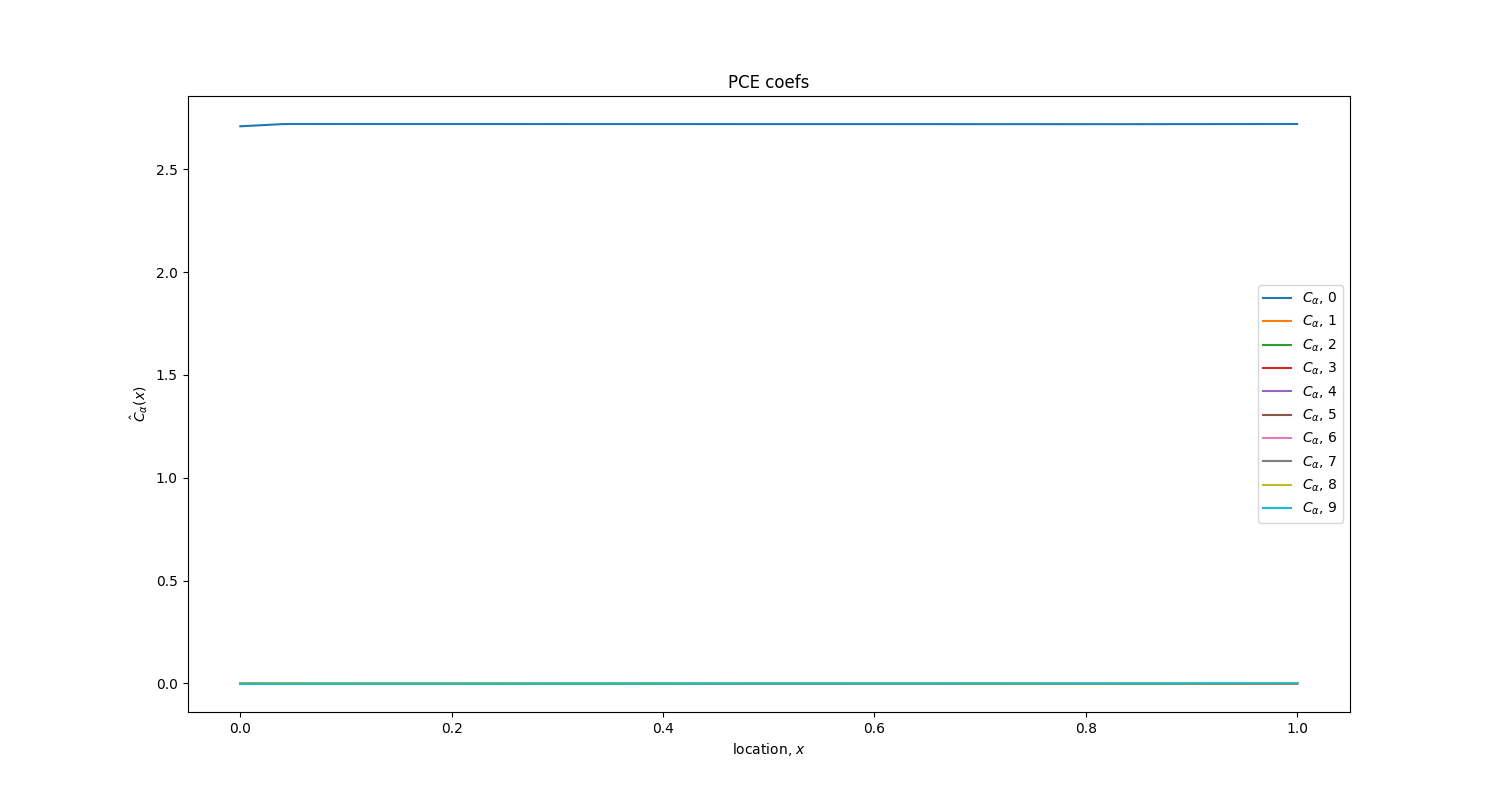
\includegraphics [trim=0 0 0 0, clip, width=0.9\textwidth, angle = 0]{figures/est_k_nn/nn_pce_coefs}
    \subcaption{Learned PCE coefficients.}\label{fig:est_k_nn_pce_coefs}
    \end{minipage}% 
    \\
    \begin{minipage}[b]{0.7\linewidth}
    \centering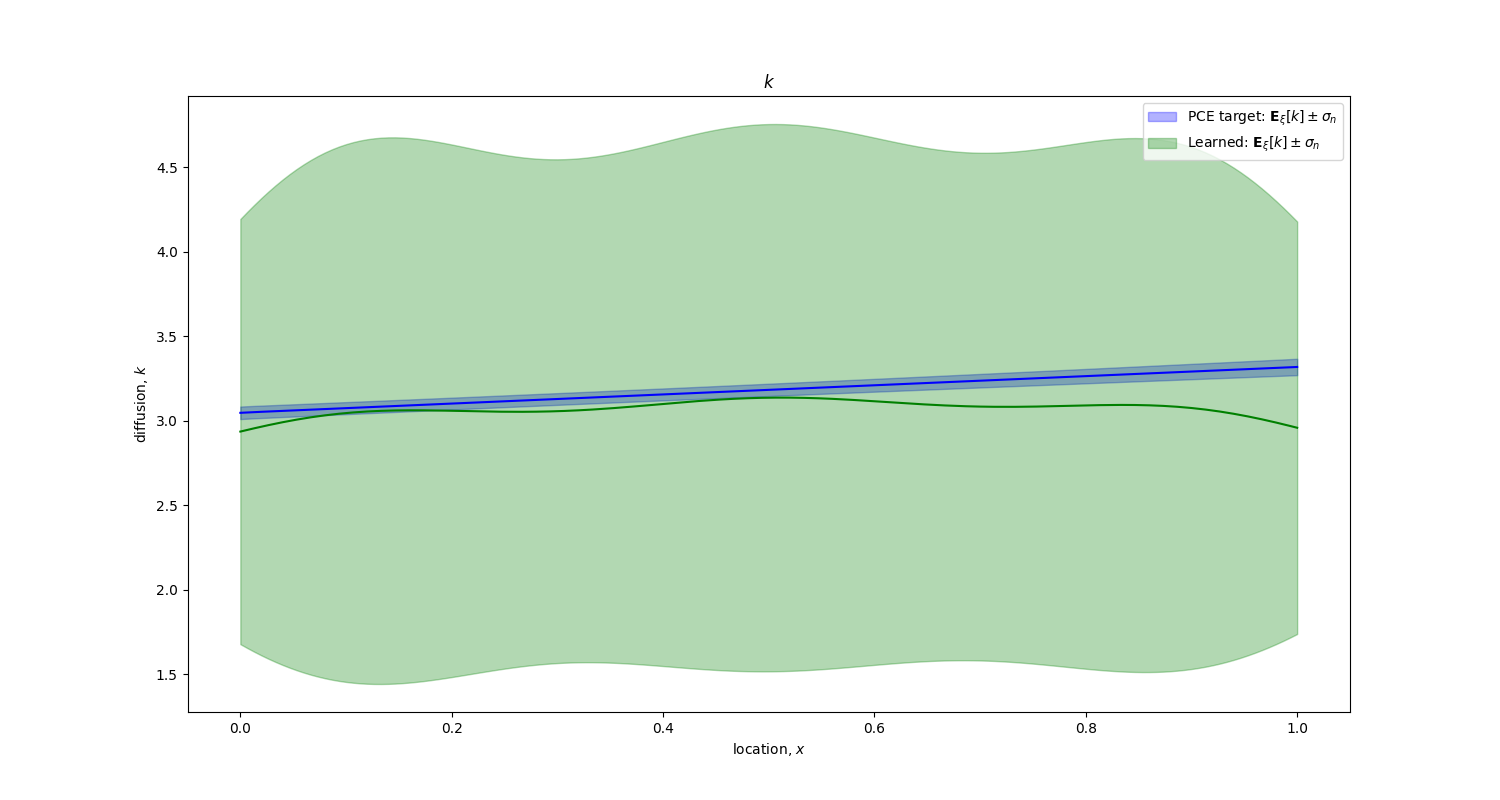
\includegraphics [trim=0 0 0 0, clip, width=0.9\textwidth, angle = 0]{figures/est_k_nn/nn_k_samples}
    \subcaption{Estimated diffusion from learned PCE coefficients.}\label{fig:est_k_nn_k}
    \end{minipage}% 
\caption{Estimated PCE coefficients (top) and diffusion, $k=\exp(Y)$ (bot) when using only diffusion, $k$, as target. The neural network approximates the correct mean $\hat \mu_k=\exp(1)$, but not the variance, $\hat \sigma_k \approx 0.005$ (note the small y-scale in bottom plot). All coefficients are zero except for the coefficient of zero-th order polynomials, $C_{[0,0,0]}$.}
\label{fig:est_k_nn}
\end{figure}
\subsection*{Learning PCE coefficients from diffusion measurements}
Training the neural network to approximate the diffusion enables us to incorporate the measurements, $k_\text{true}$, as given in project 3. As expected, the resulting curve closely matches the mean, but not the variance, as shown in~\cref{fig:est_k_true_nn} 
\begin{figure}[t]
    \centering
    \begin{minipage}[b]{0.7\linewidth}
    \centering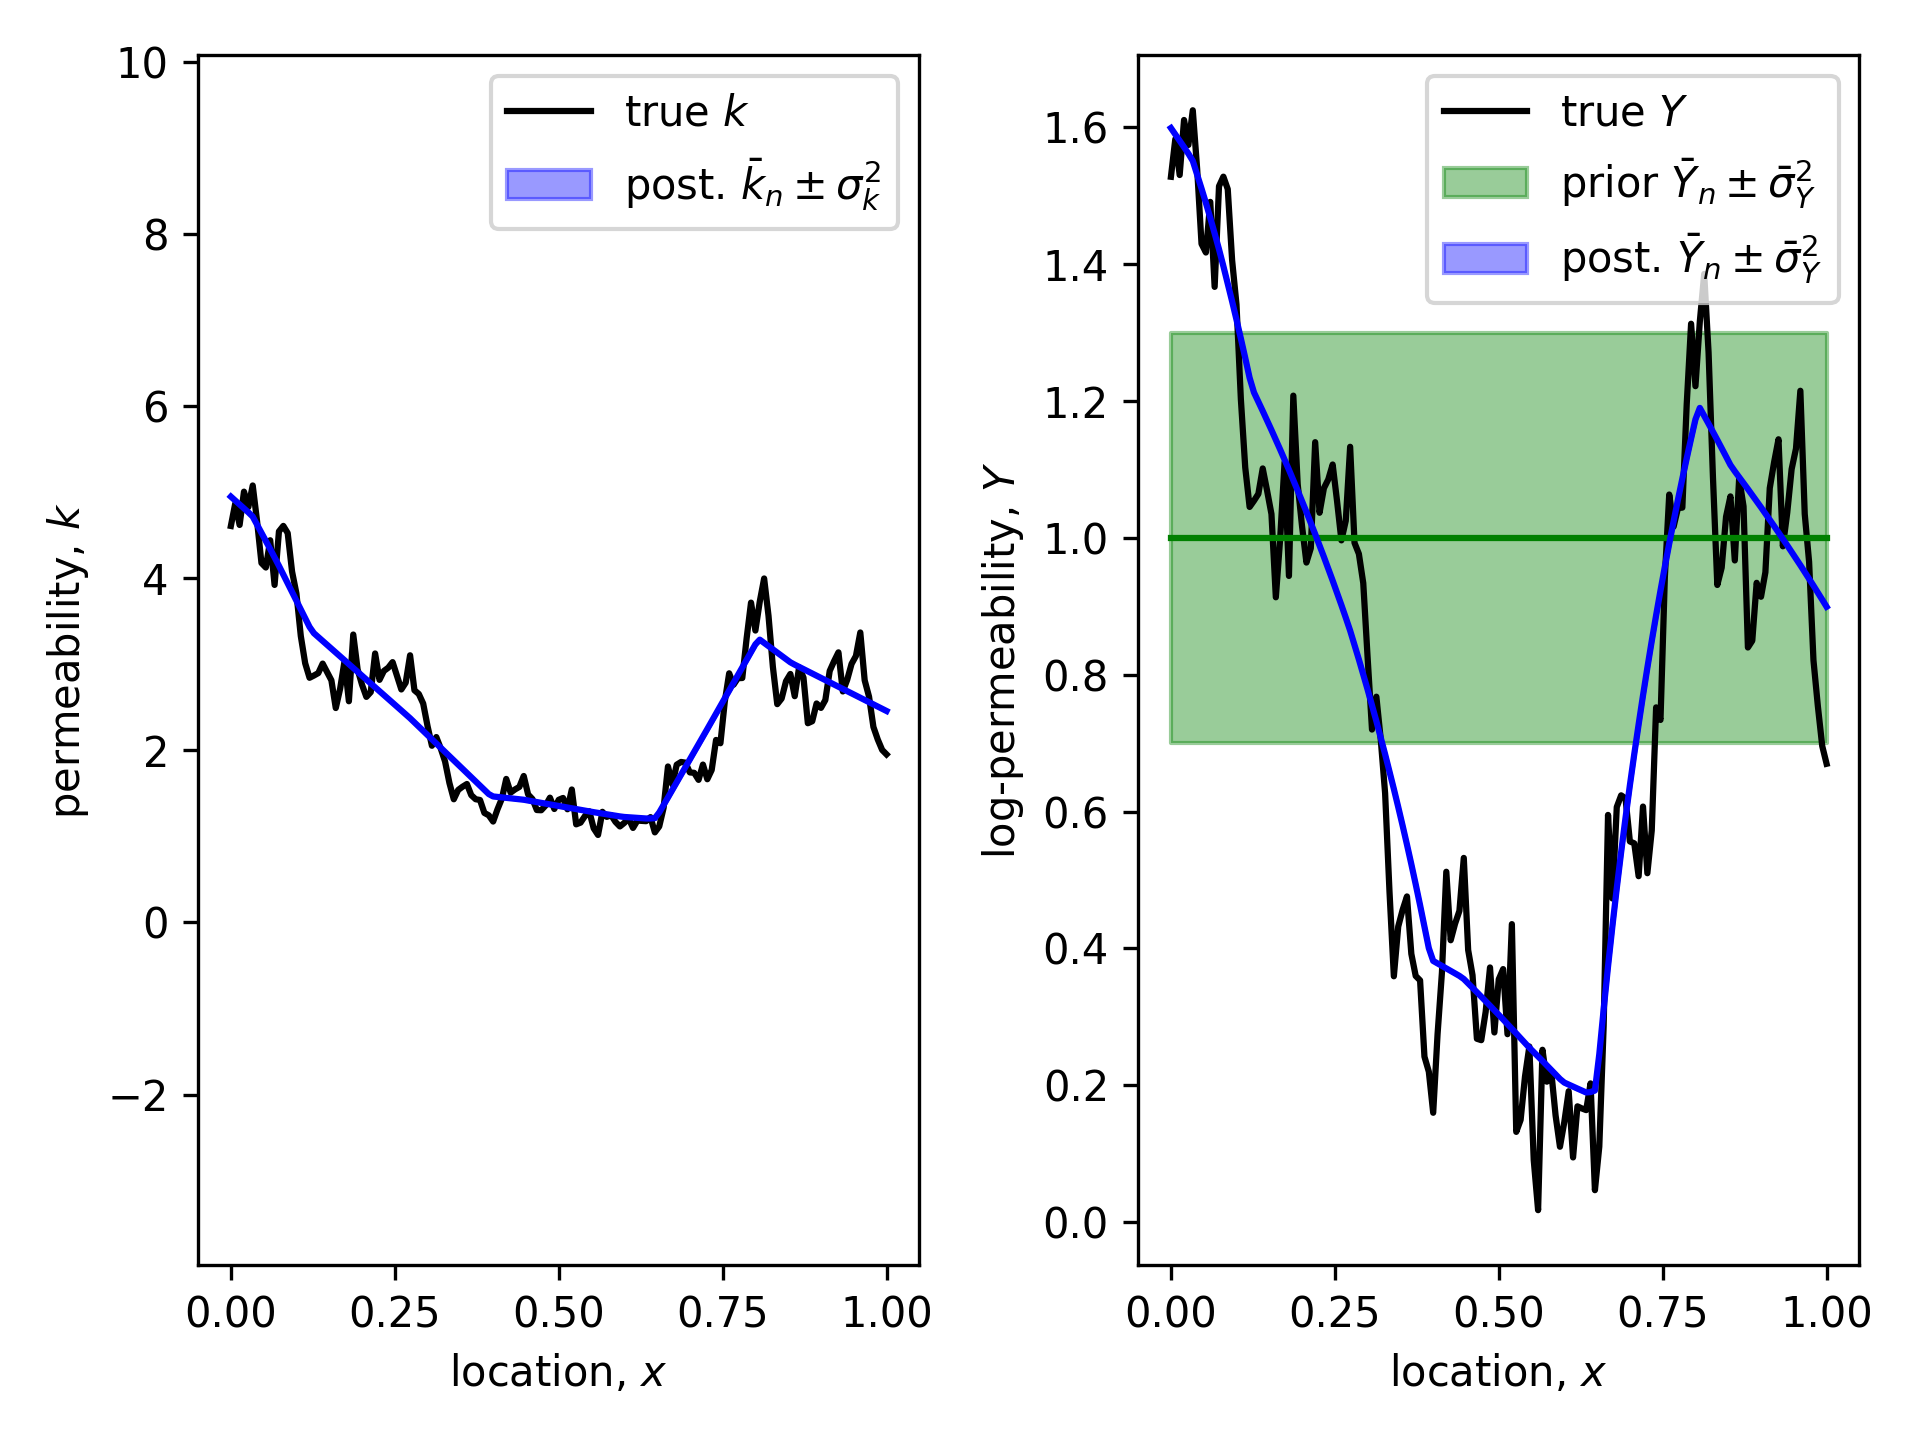
\includegraphics [trim=0 0 0 0, clip, width=0.9\textwidth, angle = 0]{figures/est_k_true_nn/k_gp_vs_msmts}
    \end{minipage}% 
\caption{Estimated diffusion, $k=\exp(Y)$ when using diffusion measurements, $k_\text{true}$ (black), as target. The neural network (blue) approximates the correct mean, but not the variance. The prior, $k$, (green) is shown but not used.}
\label{fig:est_k_true_nn}
\end{figure}
\section{Future work}
\subsection{Physics-Informed Neural Networks}
The current work aims to approximate uncertainty by estimating the PCE coefficients from measurements of the diffusion, $k$. In practice, we might not be able to measure, $k$, and might want to infer PCE coefficients from measurements of the solution, $u$. In this case, the loss function per training sample, $b$, becomes: 
\begin{equation}
\begin{aligned}
  L_{u,e,b} &= \lvert\lvert u_{e,b} - \hat u\rvert\rvert_2^2\\
  &= \lvert\lvert u_{e,b} - \text{ODEsolve}[\frac{\delta}{\delta x}(\hat k(x,\vec\xi)\frac{\delta u(x, \vec\xi)}{\delta x})]\rvert\rvert_2^2\\
  \text{with}&\\
  \hat k(x, \vec\xi)&= \lvert\lvert (\exp(\sum_{\vec\alpha \in A} \hat C_{\vec\alpha}(x_b)\Psi_{\vec\alpha}(\xi_1, ..., \xi_n))]\rvert\rvert_2^2\\
\end{aligned}
\label{eq:loss_k}
\end{equation}
Including the solver of ordinary differential equations, ODEsolve, in the loss function, however, introduces the problem of high memory complexity and numerical instability:

\textbf{Memory complexity.} The loss needs to backpropagated through ODEsolve to compute the gradient wrt. the loss of each network weight, $\theta$. In \cref{sec:coef_data} this was possible by reverse-mode automatic differentiation~\cite{Baydin_2017}. Automatic differentiation is constant in time over the size of input features, which made is successful for training very large neural networks. However, the time and memory scales linearly with the number of operations (as the symbolic derivative of each elementary operation is stored). Numerical differential equation solvers can consist of many steps, which makes the computation of gradients computationally expensive. Recent works achieve a drastic reduction in computational complexity by leveraging the implicit function theorem \cite{Li_2020}.

\textbf{Numerical instability.} There currently is no guarantee that ODEsolve finds a solution, $u$, for every diffusion parameter that the neural network estimates. More work needs to be done in bounding the neural network output to feasible parameters.

%Backpropagation through ODEsolve is computationally and storage-wise very expensive and numerically instable, because it calculates the gradient for every step in the numerical solution scheme. Alternatively $http://implicit-layers-tutorial.org/implicit_functions/$ shows, via the implicit function theorem, that the gradient can be computed by implicit differentiation by (1) computing the solution and (2) then essentially linearizing the function at the solution/fixed point and then solving a system of linear equation. I think, the key equation is $w^T\delta z^*(a_0) = w^T[I - \delta_1 f(a_0, z_0)]^{-1}\delta_0 f(a_0,z_0)$ 



\subsection{Model Uncertainty}
Neural networks can fail to extrapolate beyond the training data~\cite{Amodei_2016}. It might be possible to identify poor predictive performance via high predictive uncertainty estimates, but deep neural networks do not readily quantify predictive uncertainty~\cite{Amodei_2016,Gal_2016b}. Hence, neural network-based subgrid parametrizations might not be trustworthy due to possible errors in the prediction and the lack of the respective uncertainty. 

Luckily,~\cite{Zhang_2019} proposes the quantification of model uncertainty in neural networks via an approximation of inference in deep Gaussian Processes, called MC-Dropout~\cite{Gal_2016}. A follow-up work, however, showed that uncertainty estimates from Bayesian Neural Networks (BNNs), trained via HMC, are significantly more accurate than the MC-dropout-based uncertainty estimates~\cite{Yanga_2021}. Unfortunately, BNNs are in comparison to MC-dropout uncertainty less scalable to very large neural networks. Future work, will investigate accurate and scalable estimates of model uncertainty, such as deep ensembles which trains an ensemble of deterministic neural networks on overlapping samples of the training dataset~\cite{Lakshinarayanan_2017}. 

The first step in evaluating model uncertainty would be to measure the PCE coefficients at few locations, $x$, and then show high/low variance in between/on the sampling locations, respectively. In the next experiment one could sample stochastic, $k$, with high/low variance and evaluate if the predicted model uncertainty is higher/lower. 

\subsection{Climate Modeling}
The current work dealt with a simple 1D elliptic stochastic diffusion equation. Future work, will investigate more complicated partial differential equations. For example, a stochastic advection-diffusion equation, or the system of Rayleigh-Benard convection equations~\cite{Emanuel_1995}. 

\clearpage

%\addtolength{\textheight}{-12cm}   % This command serves to balance the column lengths
%                                  % on the last page of the document manually. It shortens
%                                  % the textheight of the last page by a suitable amount.
%                                  % This command does not take effect until the next page
%                                  % so it should come on the page before the last. Make
%                                  % sure that you do not shorten the textheight too much.%

%%%%%%%%%%%%%%%%%%%%%%%%%%%%%%%%%%%%%%%%%%%%%%%%%%%%%%%%%%%%%%%%%%%%%%%%%%%%%%%%



%%%%%%%%%%%%%%%%%%%%%%%%%%%%%%%%%%%%%%%%%%%%%%%%%%%%%%%%%%%%%%%%%%%%%%%%%%%%%%%%



%%%%%%%%%%%%%%%%%% %%%%%%%%%%%%%%%%%%%%%%%%%%%%%%%%%%%%%%%%%%%%%%%%%%%%%%%%%%%%%%
\section*{ACKNOWLEDGMENT}

The author is very grateful for the preparation and lecture of the material by Prof. Youssef Marzouk and continuous help and feedback in office hours by the teaching assistants, Fengyi Lu, Michael Brennan, and Andrea Scarinci.
%%%%%%%%%%%%%%%%%%%%%%%%%%%%%%%%%%%%%%%%%%%%%%%%%%%%%%%%%%%%%%%%%%%%%%%%%%%%%%%%
%\clearpage

%(including class)
\balance
\bibliographystyle{IEEEtran} 
% \bibliographystyle{unsrt} 
\bibliography{biblio}


\end{document}
